\chapter{Zuren en basen: Ka en pKa}\label{ch:g12:ka-and-pka}

Veel mieren verdedigen zich met methaanzuur, en op de huid brandt het.
Methaanzuur is een klein
\omterm{def:g11:functional-groups:carboxylic-acid}{carbonzuur}. Zoutzuur van dezelfde concentratie zou veel erger branden.
Allebei zijn het zuren; allebei geven ze een oplossing met een \omterm{def:g9:acids-bases-ph:ph}{pH} onder 7;
toch zijn ze niet op dezelfde manier zuur. Om een zuur volledig te
beschrijven, zijn twee getallen nodig: hoeveel ervan er is, de
concentratie, en hoe gemakkelijk het zijn waterstofion afstaat, de
\omterm{def:g12:ka-and-pka:ka}{zuurconstante}.

\begin{recall}
Zure, basische en \omterm{def:g9:acids-bases-ph:acidic}{neutrale oplossingen}; de pH-schaal, van 0 tot 14, lager
als er meer waterstofionen zijn (\cref{ch:g9:acids-bases-ph}). Het
\omterm{def:g12:equilibrium:quotient}{reactiequotiënt} $Q$ en de \omterm{def:g12:equilibrium:constant}{evenwichtsconstante} $K$
(\cref{ch:g12:equilibrium}). Een \omterm{def:g12:curly-arrows:curly-arrow}{gebogen pijl} laat een elektronenpaar zien
dat zich verplaatst (\cref{ch:g12:curly-arrows}).
\end{recall}

\begin{omfigure}
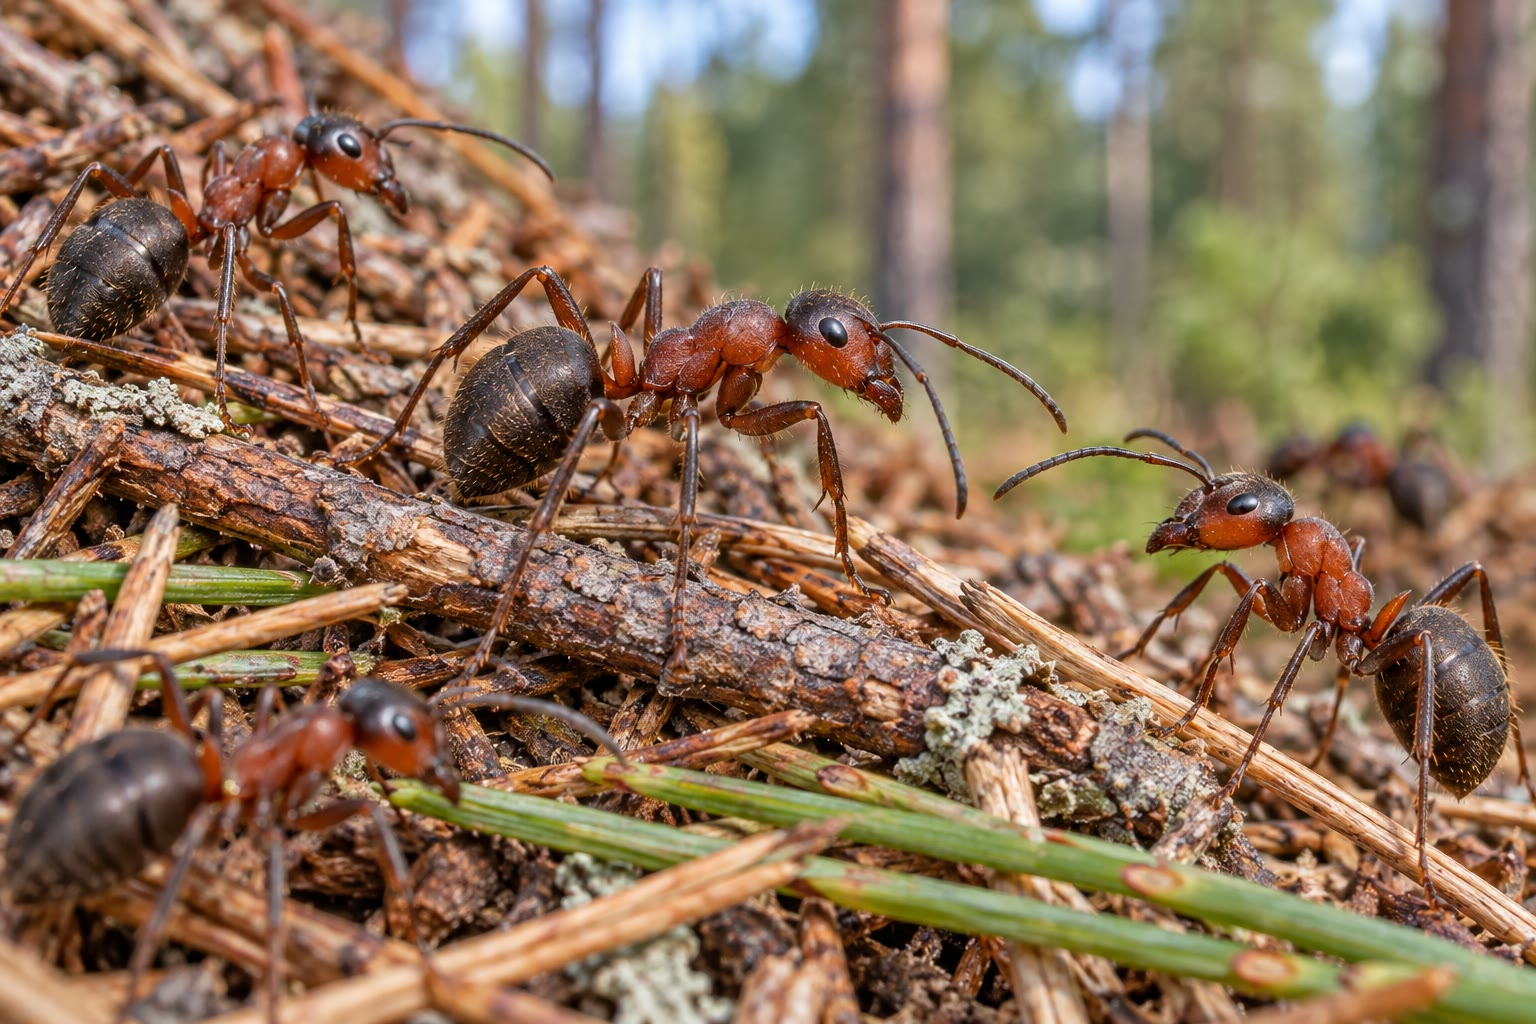
\includegraphics[width=0.45\linewidth]{images/book1/ai/g12-red-ants.jpg}

{\small Rode bosmieren: zoals veel mieren verdedigen ze zich met
methaanzuur.}
\end{omfigure}

\section{Zuren en basen volgens Brønsted}

\begin{definition}[Zuur en base volgens Brønsted, zuur-basekoppel]\label{def:g12:ka-and-pka:bronsted}
Een \emph{zuur volgens Brønsted}\index{zuur volgens Brønsted} is een
deeltje dat een waterstofion \ce{H+} kan afstaan; een \emph{base volgens
Brønsted}\index{base volgens Brønsted} is een deeltje dat er een kan
opnemen. Een zuur HA en de base \ce{A-} die het wordt door \ce{H+} af te
staan, vormen een \emph{zuur-basekoppel}\index{zuur-basekoppel},
geschreven als \ce{HA}/\ce{A-}: $\ce{HA} \rightleftharpoons \ce{A-} + \ce{H+}$.
\end{definition}

\begin{definition}[Oxoniumion, amfolyt]\label{def:g12:ka-and-pka:oxonium}
In water blijft een waterstofion nooit alleen: een watermolecuul neemt het
op, en zo ontstaat het \emph{oxoniumion}\index{oxoniumion} \ce{H3O+}. Een
deeltje dat het zuur is van het ene koppel en de base van een ander, is
een \emph{amfolyt}\index{amfolyt}; water is er een, zuur van het koppel
\ce{H2O}/\ce{OH-} en base van het koppel \ce{H3O+}/\ce{H2O}.
\end{definition}

\begin{example}[Een zuur in water]\label{ex:g12:ka-and-pka:acid-water}
Als ethaanzuur \omterm{def:g2:mixing-and-dissolving:dissolve}{oplost}, neemt een \omterm{def:g10:lewis-and-shape:lone-pair}{vrij elektronenpaar} van een watermolecuul
het waterstofatoom van zijn \ce{O-H} over, en het \ce{O-H}-paar blijft op
het zuurstofatoom van het zuur:
\[
  \ce{CH3COOH + H2O <=> CH3COO- + H3O+} .
\]
Twee koppels wisselen een waterstofion uit: \ce{CH3COOH}/\ce{CH3COO-}
staat het af, \ce{H3O+}/\ce{H2O} neemt het op. Vanaf nu worden de
waterstofionen van eerdere hoofdstukken als \ce{H3O+} geschreven als water
het \omterm{def:g6:solutions-and-solubility:solute}{oplosmiddel} is.
\end{example}

\begin{omfigure}
\setchemfig{atom sep=2em}
\chemfig{H_3C-C(=[2]O)-O-[@{oh}]@{h}H}\qquad
\chemfig{@{ow}\charge{90=\:,270=\:}{O}(-[:150]H)-[:210]H}
\qquad$\longrightarrow$\qquad
\chemfig{H_3C-C(=[2]O)-\charge{90=\:,0=\:,270=\:}{O}^{-}}\quad$+$\quad\ce{H3O+}
\chemmove{
  \draw[->, thick, omProp, shorten <=4pt, shorten >=3pt]
    ($(ow)+(0,0.25)$) .. controls +(110:9mm) and +(60:9mm) .. (h);
  \draw[->, thick, omDef, shorten <=2pt, shorten >=4pt]
    (oh) .. controls +(-90:7mm) and +(-60:6mm) .. ($(oh)+(-0.3,-0.2)$);}

{\small Een waterstofion gaat over van het zuur naar water: een \omterm{def:g10:lewis-and-shape:lone-pair}{vrij
elektronenpaar} van water vormt de nieuwe \ce{O-H}-binding (oranje), en
het oude \ce{O-H}-paar blijft op het zuurstofatoom van het ethanoaation
(blauw).}
\end{omfigure}

\begin{history}[Van Arrhenius naar Brønsted, 1887--1923]
In 1887 stelde Svante Arrhenius voor dat zuren in water waterstofionen
geven en basen \omterm{def:g9:ions:ion}{hydroxide-ionen}. In 1923 verbreedden Johannes Brønsted
en, onafhankelijk van hem, Thomas Lowry dat idee: een zuur is elk deeltje
dat een waterstofion afstaat, een base elk deeltje dat er een opneemt, in
water of niet. Het ammoniakmolecuul, dat geen hydroxide bevat, werd een
base als elke andere.
\end{history}

\begin{omfigure}
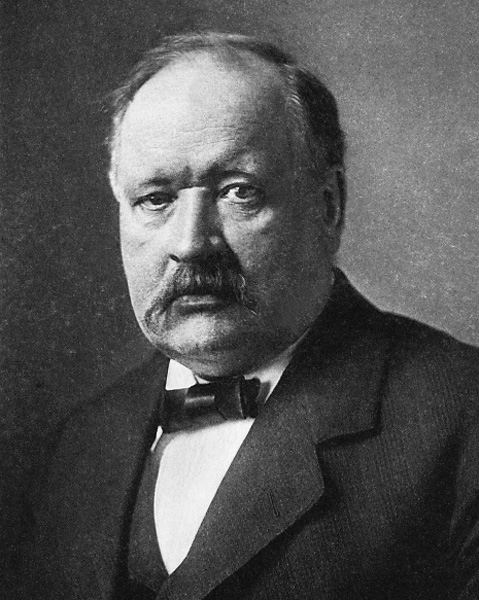
\includegraphics[width=0.22\linewidth]{images/book1/arrhenius.jpg}

{\small Svante Arrhenius (1859--1927).}
\end{omfigure}

\section{De pH, kwantitatief}

\begin{definition}[De pH, precies]\label{def:g12:ka-and-pka:ph-log}
In een verdunde \omterm{def:g6:solutions-and-solubility:solute}{waterige oplossing} is de \omterm{def:g9:acids-bases-ph:ph}{pH} gedefinieerd door
\[
  \mathrm{pH} = -\log\frac{[\ce{H3O+}]}{c^\circ},
  \qquad\text{dat wil zeggen}\qquad
  [\ce{H3O+}] = c^\circ \times 10^{-\mathrm{pH}} ,
\]
waarin $\log$ de briggse logaritme is.
\end{definition}

\begin{proposition}[Tien keer verdunnen, één eenheid]\label{prop:g12:ka-and-pka:dilution}
Als $[\ce{H3O+}]$ door 10 gedeeld wordt, stijgt de \omterm{def:g9:acids-bases-ph:ph}{pH} met 1; als het met
10 vermenigvuldigd wordt, daalt de \omterm{def:g9:acids-bases-ph:ph}{pH} met 1.
\end{proposition}

\begin{proof}
$-\log\big([\ce{H3O+}]/10c^\circ\big) = -\log\big([\ce{H3O+}]/c^\circ\big)
+ \log 10 = \mathrm{pH} + 1$.
\end{proof}


\begin{definition}[Sterke en zwakke zuren en basen]\label{def:g12:ka-and-pka:strong-acid}
Een \emph{sterk zuur}\index{sterk zuur} reageert volledig met water: er
blijft niets van het zuur als zodanig in de oplossing over. Een
\emph{zwak zuur}\index{zwak zuur} reageert gedeeltelijk: zijn reactie met
water bereikt een evenwicht. Zo reageert ook een \emph{sterke
base}\index{sterke base} volledig met water, en een \emph{zwakke
base}\index{zwakke base} gedeeltelijk.
\end{definition}

\begin{proposition}[pH van een sterk zuur]\label{prop:g12:ka-and-pka:strong}
Een oplossing van een \omterm{def:g12:ka-and-pka:strong-acid}{sterk zuur} met concentratie $c$ (niet te verdund)
heeft $[\ce{H3O+}] = c$ en $\mathrm{pH} = -\log(c/c^\circ)$.
\end{proposition}

\begin{proof}
De reactie \ce{HA + H2O -> A- + H3O+} is aflopend: elk \omterm{def:g7:atoms-and-molecules:molecule}{molecuul} zuur
geeft één \omterm{def:g12:ka-and-pka:oxonium}{oxoniumion}. De \omterm{def:g9:ions:ion}{ionen} die uit het water zelf komen, zijn
verwaarloosbaar zolang $c$ veel groter is dan \qty{e-7}{mol/L}.
\end{proof}

\begin{example}[Zoutzuur]\label{ex:g12:ka-and-pka:hcl}
Neem zoutzuur van \qty{0.010}{mol/L}: daarin is
$[\ce{H3O+}] = \qty{0.010}{mol/L}$ en $\mathrm{pH} = -\log 0.010 = 2.0$. Tien keer verdund: \omterm{def:g9:acids-bases-ph:ph}{pH} 3.0.
\end{example}

\section{Water en het ionenproduct}


\begin{definition}[Ionenproduct van water]\label{def:g12:ka-and-pka:ionic-product}
Water reageert in heel geringe mate met zichzelf,
\ce{2H2O <=> H3O+ + OH-}. De \omterm{def:g12:equilibrium:constant}{evenwichtsconstante} van deze reactie is het
\emph{ionenproduct van water}\index{ionenproduct van water}:
\[
  K_e = \frac{[\ce{H3O+}]\,[\ce{OH-}]}{(c^\circ)^2},
  \qquad pK_e = -\log K_e .
\]
\end{definition}

\begin{proposition}[Neutraal water en sterke basen]\label{prop:g12:ka-and-pka:ke}
% ledger: ke:25C
Bij \qty{25}{\celsius} is $K_e = \num{1.0e-14}$ en $pK_e = 14.0$. In
zuiver water is $[\ce{H3O+}] = [\ce{OH-}] = \qty{1.0e-7}{mol/L}$: \omterm{def:g9:acids-bases-ph:ph}{pH} 7.0.
Een \omterm{def:g12:ka-and-pka:strong-acid}{sterke base} met concentratie $c$ geeft $[\ce{OH-}] = c$, dus
$[\ce{H3O+}] = K_e (c^\circ)^2 / c$ en $\mathrm{pH} = 14.0 + \log(c/c^\circ)$.
\end{proposition}

\begin{proof}
In zuiver water ontstaan de twee \omterm{def:g9:ions:ion}{ionen} in paren, dus ze zijn even groot,
en hun product is $\num{1.0e-14}$: elk is \qty{1.0e-7}{mol/L}. Voor de
base geldt $K_e$ nog steeds in de oplossing:
$-\log([\ce{H3O+}]/c^\circ) = -\log K_e + \log(c/c^\circ)$.
\end{proof}

\begin{example}[Natronloog]\label{ex:g12:ka-and-pka:naoh}
Natronloog van \qty{0.010}{mol/L}: $[\ce{OH-}] = 0.010$, dus
$[\ce{H3O+}] = \num{1.0e-14}/0.010 = \qty{1.0e-12}{mol/L}$ en \omterm{def:g9:acids-bases-ph:ph}{pH} 12.0.
\end{example}

\section{De zuurconstante}

\begin{definition}[Zuurconstante, $pK_a$]\label{def:g12:ka-and-pka:ka}
De \emph{zuurconstante}\index{zuurconstante} $K_a$ van een koppel
\ce{HA}/\ce{A-} is de \omterm{def:g12:equilibrium:constant}{evenwichtsconstante} van de reactie van het zuur met
water, \ce{HA + H2O <=> A- + H3O+}:
\[
  K_a = \frac{[\ce{A-}]\,[\ce{H3O+}]}{[\ce{HA}]\,c^\circ} .
\]
De \emph{pKa}\index{pKa} van het koppel is
$pK_a = -\log K_a$.
\end{definition}

\begin{proposition}[Hoe kleiner de $pK_a$, hoe sterker het zuur]\label{prop:g12:ka-and-pka:compare}
Van twee \omterm{def:g12:ka-and-pka:strong-acid}{zwakke zuren} met dezelfde concentratie reageert het zuur met de
grootste $K_a$, dus de kleinste $pK_a$, het meest met water en geeft het
de laagste \omterm{def:g9:acids-bases-ph:ph}{pH}; zijn geconjugeerde base is de zwakste.
\end{proposition}

\begin{proof}
Een grotere $K_a$ betekent meer \ce{A-} en \ce{H3O+} in evenwicht bij
dezelfde \ce{HA}. De base \ce{A-} van een koppel dat zijn waterstofion
gemakkelijk afstaat, neemt het maar met moeite terug.
\end{proof}

\begin{omfigure}
\begin{tikzpicture}[font=\small, y=0.55cm]
  % ledger: pka:methanoic, pka:ethanoic, pka:benzoic, pka:ascorbic1, ka:HF, ka:H2CO3, ka:HCO3, kb:NH3, ke:25C
  \draw[->, thick] (0,0) -- (0,14.8) node[above] {$pK_a$};
  \foreach \k in {0,2,4,6,8,10,12,14} \draw (-0.1,\k) -- (0.1,\k) node[right, font=\scriptsize] {\k};
  \node[font=\footnotesize\bfseries, anchor=south] at (-3.0,14.3) {zuur};
  \node[font=\footnotesize\bfseries, anchor=south] at (3.0,14.3) {base};
  \foreach \p/\yl/\acid/\base in {3.19/2.9/{\ce{HF}}/{\ce{F-}},
      3.74/3.6/{\ce{HCOOH}}/{\ce{HCOO-}}, 4.04/4.3/{ascorbinezuur}/{ascorbaat},
      4.20/5.0/{\ce{C6H5COOH}}/{\ce{C6H5COO-}}, 4.76/5.7/{\ce{CH3COOH}}/{\ce{CH3COO-}},
      6.37/6.9/{\ce{CO2,H2O}}/{\ce{HCO3-}}, 9.26/9.26/{\ce{NH4+}}/{\ce{NH3}},
      10.33/10.4/{\ce{HCO3-}}/{\ce{CO3^{2-}}}} {
    \draw[omDef] (-0.25,\p) -- (0.25,\p);
    \draw[black!40] (-0.25,\p) -- (-1.1,\yl);
    \draw[black!40] (0.25,\p) -- (1.1,\yl);
    \node[anchor=east, font=\scriptsize] at (-1.15,\yl) {\acid};
    \node[anchor=west, font=\scriptsize] at (1.15,\yl) {\base};
  }
  \draw[->, omThm, thick] (-4.6,13) -- (-4.6,1);
  \node[omThm, rotate=90, font=\footnotesize] at (-4.95,7) {sterkere zuren};
  \draw[->, omMeth, thick] (4.6,1) -- (4.6,13);
  \node[omMeth, rotate=90, font=\footnotesize] at (4.95,7) {sterkere basen};
\end{tikzpicture}

{\small Enkele koppels, gerangschikt naar hun $pK_a$ bij
\qty{25}{\celsius}, zuren links, hun basen rechts. Hoe lager een koppel op
de schaal, hoe sterker zijn zuur; hoe hoger, hoe sterker zijn base.}
\end{omfigure}


\begin{method}[pH van een zwak zuur]\label{met:g12:ka-and-pka:weak}
Voor een \omterm{def:g12:ka-and-pka:strong-acid}{zwak zuur} met concentratie $c$ en constante $K_a$:
\begin{enumerate}
  \item Stel de \omterm{def:g10:reaction-progress-table:extent}{voortgangstabel} op van \ce{HA + H2O <=> A- + H3O+} per
        liter,
        met $x = [\ce{H3O+}]$: $[\ce{HA}] = c - x$, $[\ce{A-}] = x$
        (de eigen \omterm{def:g9:ions:ion}{ionen} van water verwaarloosd).
  \item Los $\dfrac{x^2}{(c - x)\,c^\circ} = K_a$ op, de
        vierkantsvergelijking
        $x^2 + K_a c^\circ x - K_a c^\circ c = 0$, en houd de positieve
        wortel.
  \item $\mathrm{pH} = -\log(x/c^\circ)$; controleer dat $x$ veel groter
        is dan \qty{e-7}{mol/L}.
\end{enumerate}
\end{method}

\begin{example}[Ethaanzuur van \texorpdfstring{\qty{0.010}{mol/L}}{0.010 \omterm{def:g10:the-mole:amount}{mol}/L}]\label{ex:g12:ka-and-pka:acetic}
% ledger: pka:ethanoic
$pK_a = 4.76$, dus $K_a = 10^{-4.76} = \num{1.74e-5}$. Dan geeft
$x^2 + \num{1.74e-5}\,x - \num{1.74e-7} = 0$
$x = \qty{4.1e-4}{mol/L}$ en \omterm{def:g9:acids-bases-ph:ph}{pH} 3.39. Slechts $\num{4.1e-4}/0.010 =
\qty{4.1}{\percent}$ van het zuur heeft met water gereageerd; zoutzuur van
dezelfde concentratie, \omterm{def:g9:acids-bases-ph:ph}{pH} 2.0, heeft volledig gereageerd.
\end{example}

\begin{omfigure}
\begin{tikzpicture}[font=\small]
  \fill[omThm!45] (0,1.3) rectangle (8,2.0);
  \node[anchor=east] at (-0.1,1.65) {\ce{HCl}, \qty{0.010}{mol/L}};
  \node[white, font=\small\bfseries] at (4,1.65) {\ce{H3O+} + \ce{Cl-}: \qty{100}{\percent}};
  \fill[omDef!35] (0,0) rectangle (7.67,0.7);
  \fill[omThm!45] (7.67,0) rectangle (8,0.7);
  \node[anchor=east] at (-0.1,0.35) {\ce{CH3COOH}, \qty{0.010}{mol/L}};
  \node at (3.8,0.35) {\ce{CH3COOH} als zodanig over: \qty{95.9}{\percent}};
  \draw[<-, omThm] (7.85,0.75) -- (8.4,1.1) node[right, font=\footnotesize] {\qty{4.1}{\percent} geïoniseerd};
\end{tikzpicture}

{\small Wat er gebeurt met een sterk en een \omterm{def:g12:ka-and-pka:strong-acid}{zwak zuur} van dezelfde
concentratie: het \omterm{def:g12:ka-and-pka:strong-acid}{sterke zuur} wordt helemaal omgezet in \omterm{def:g9:ions:ion}{ionen}, het \omterm{def:g12:ka-and-pka:strong-acid}{zwakke
zuur} nauwelijks. Vandaar het verschil in \omterm{def:g9:acids-bases-ph:ph}{pH}, 2.0 tegen 3.4.}
\end{omfigure}

\begin{safety}{\ghs[0.75cm]{GHS02}\ghs[0.75cm]{GHS05}\ghs[0.75cm]{GHS06}\ghs[0.75cm]{GHS07}}
% ledger: ghs:formic-acid
Geconcentreerd methaanzuur is ontvlambaar, veroorzaakt ernstige
brandwonden aan huid en ogen, en de damp ervan is giftig. Alleen de
docent werkt ermee, in een zuurkast; ook de verdunde oplossingen van de
oefeningen vragen om een veiligheidsbril.
\end{safety}

\section{Oefeningen}

\begin{exercise}[$\star$]\label{exo:g12:ka-and-pka:1}
Geef de geconjugeerde base van: \ce{HCOOH}, \ce{NH4+}, \ce{H2O},
\ce{HCO3-}; en het geconjugeerde zuur van: \ce{NH3}, \ce{OH-}, \ce{H2O},
\ce{HCO3-}. Welke deeltjes zijn \omterm{def:g12:ka-and-pka:oxonium}{amfolyten}?
\end{exercise}

\begin{exercise}[$\star$]\label{exo:g12:ka-and-pka:2}
Bereken de \omterm{def:g9:acids-bases-ph:ph}{pH} van zoutzuur van \qty{0.10}{mol/L},
\qty{0.0010}{mol/L} en \qty{5.0e-3}{mol/L}.
\end{exercise}

\begin{exercise}[$\star$]\label{exo:g12:ka-and-pka:3}
Een oplossing heeft \omterm{def:g9:acids-bases-ph:ph}{pH} 4.5. Bereken $[\ce{H3O+}]$. Een oplossing heeft
\omterm{def:g9:acids-bases-ph:ph}{pH} 11.2: bereken $[\ce{H3O+}]$ en $[\ce{OH-}]$ bij \qty{25}{\celsius}.
\end{exercise}

\begin{exercise}[$\star$]\label{exo:g12:ka-and-pka:4}
Schrijf de reactie met water en de uitdrukking voor $K_a$ op voor
methaanzuur en voor het ammoniumion.
\end{exercise}

\begin{exercise}[$\star$]\label{exo:g12:ka-and-pka:5}
Welk zuur is het sterkst: methaanzuur ($pK_a = 3.74$) of ethaanzuur
($pK_a = 4.76$)? Welke base is het sterkst: \ce{HCOO-} of
\ce{CH3COO-}?
\end{exercise}

\begin{exercise}[$\star\star$]\label{exo:g12:ka-and-pka:6}
Een oplossing van een \omterm{def:g12:ka-and-pka:strong-acid}{zwak zuur} HA van \qty{0.050}{mol/L} heeft \omterm{def:g9:acids-bases-ph:ph}{pH} 3.0.
Bereken $[\ce{A-}]$, $[\ce{HA}]$, en daarna $K_a$ en $pK_a$.
\end{exercise}

\begin{exercise}[$\star\star$]\label{exo:g12:ka-and-pka:7}
Bereken de \omterm{def:g9:acids-bases-ph:ph}{pH} van benzoëzuur van \qty{0.020}{mol/L} ($pK_a = 4.20$).
\end{exercise}

\begin{exercise}[$\star\star$]\label{exo:g12:ka-and-pka:8}
Bereken de \omterm{def:g9:acids-bases-ph:ph}{pH} van natronloog van \qty{2.0e-3}{mol/L}.
\end{exercise}

\begin{exercise}[$\star\star$]\label{exo:g12:ka-and-pka:9}
Zet met de $pK_a$-schaal de zuren van de getoonde koppels op volgorde van
het sterkste naar het zwakste. Waar zou een \omterm{def:g12:ka-and-pka:strong-acid}{sterk zuur} zoals \ce{HCl}
liggen?
\end{exercise}

\begin{exercise}[$\star\star$]\label{exo:g12:ka-and-pka:10}
Koolstofdioxide dat in water is opgelost, maakt het licht zuur (koppel
\ce{CO2,H2O}/\ce{HCO3-}, $pK_a = 6.37$). Een monster regenwater dat in
contact staat met de \omterm{def:g4:air-a-mixture-of-gases:air}{lucht}, blijkt \omterm{def:g9:acids-bases-ph:ph}{pH} 5.6 te hebben. Bereken
$[\ce{H3O+}]$, en vergelijk met zuiver water.
\end{exercise}

\begin{exercise}[$\star\star$]\label{exo:g12:ka-and-pka:11}
Laat zien dat voor het koppel \ce{NH4+}/\ce{NH3} geldt
$pK_a = pK_e - pK_b$, waarin
$K_b = \num{1.8e-5}$ de constante is van \ce{NH3 + H2O <=> NH4+ + OH-}.
Bereken de $pK_a$.
\end{exercise}

\begin{exercise}[$\star\star\star$]\label{exo:g12:ka-and-pka:12}
Ethaanzuur van \qty{0.010}{mol/L} heeft \omterm{def:g9:acids-bases-ph:ph}{pH} 3.39. Bereken de \omterm{def:g9:acids-bases-ph:ph}{pH} na tien
keer verdunnen. Stijgt die met één eenheid, zoals bij een \omterm{def:g12:ka-and-pka:strong-acid}{sterk zuur}?
Leg uit.
\end{exercise}

\begin{exercise}[$\star\star\star$]\label{exo:g12:ka-and-pka:13}
Het waterstofcarbonaation is een \omterm{def:g12:ka-and-pka:oxonium}{amfolyt}. Schrijf zijn twee reacties met
water op en hun constanten, met de $pK_a$-schaal. Welke is het grootst?
Wat zegt dat over de \omterm{def:g9:acids-bases-ph:ph}{pH} van een oplossing van natriumwaterstofcarbonaat?
\end{exercise}

\begin{exercise}[$\star\star\star$]\label{exo:g12:ka-and-pka:14}
Zoutzuur van \qty{1.0e-3}{mol/L} wordt duizend keer verdund, en daarna
nog eens duizend keer. Een onzorgvuldige regel geeft \omterm{def:g9:acids-bases-ph:ph}{pH} 6, en daarna
\omterm{def:g9:acids-bases-ph:ph}{pH} 9. Waarom is \omterm{def:g9:acids-bases-ph:ph}{pH} 9 onmogelijk voor een verdund zuur? Naar welke \omterm{def:g9:acids-bases-ph:ph}{pH} gaat
de zeer verdunde oplossing?
\end{exercise}

\begin{exercise}[$\star\star\star$]\label{exo:g12:ka-and-pka:15}
Ascorbinezuur (vitamine C, $pK_a = 4.04$, $M = \qty{176.0}{g/mol}$): een
tablet van \qty{500}{mg} wordt opgelost in \qty{200}{mL} water. Bereken
de \omterm{def:g9:acids-bases-ph:ph}{pH} (neem alleen de eerste zuurfunctie in aanmerking).
\end{exercise}

\section{Probleem: Het gif van de mier}


\begin{problem}[{Weekendprobleem --- welke pH geeft het methaanzuur van
mierengif bij 0.010 mol/L, en hoe verzacht zuiveringszout de brandende
plek?}]
\label{pb:g12:ka-and-pka:1}
% ledger: src:formic-ants, pka:methanoic, ka:H2CO3, ke:25C, aw:C, aw:H, aw:O
Methaanzuur, \ce{HCOOH}, komt voor in het gif van mieren. Zijn $pK_a$ bij
\qty{25}{\celsius} is 3.74. We bestuderen een oplossing van
\qty{0.010}{mol/L} en vergelijken die met zoutzuur.

\medskip
\noindent\textbf{Deel I --- Het zuur.}
\begin{enumerate}
  \item Teken de \omterm{def:g10:lewis-and-shape:lewis-structure}{lewisstructuur} van methaanzuur en omcirkel het
        waterstofatoom dat het afstaat.
  \item Schrijf zijn koppel op en zijn reactie met water.
  \item Schrijf $K_a$ op en bereken de waarde ervan.
  \item Plaats het koppel op de $pK_a$-schaal: is methaanzuur sterker of
        zwakker dan ethaanzuur?
  \item Bereken de massa methaanzuur in \qty{1.0}{L} van de oplossing.
\end{enumerate}

\medskip
\noindent\textbf{Deel II --- De \omterm{def:g9:acids-bases-ph:ph}{pH}.}
\begin{enumerate}[resume]
  \item Vul de \omterm{def:g10:reaction-progress-table:extent}{voortgangstabel} per liter in, met $x = [\ce{H3O+}]$.
  \item Schrijf de vergelijking $Q_{eq} = K_a$ op.
  \item Los haar op.
  \item Bereken de \omterm{def:g9:acids-bases-ph:ph}{pH}.
  \item Welk deel van het zuur heeft met water gereageerd?
  \item Controleer dat je de \omterm{def:g9:ions:ion}{ionen} uit het water kunt verwaarlozen.
\end{enumerate}

\medskip
\noindent\textbf{Deel III --- Vergelijking.}
\begin{enumerate}[resume]
  \item Wat is de \omterm{def:g9:acids-bases-ph:ph}{pH} van zoutzuur van \qty{0.010}{mol/L}?
  \item Hoeveel keer meer \omterm{def:g12:ka-and-pka:oxonium}{oxoniumionen} bevat het dan de oplossing van
        methaanzuur?
  \item Verklaar het verschil met de woorden sterk en zwak.
\end{enumerate}

\medskip
\noindent\textbf{Deel IV --- Zuiveringszout.}
\begin{enumerate}[resume]
  \item Zuiveringszout is natriumwaterstofcarbonaat. Schrijf de reactie
        op tussen methaanzuur en het waterstofcarbonaation (ze geeft
        methanoaat en \ce{CO2,H2O}).
  \item Laat zien dat haar constante $K = K_a(\ce{HCOOH}) / K_a(\ce{CO2,H2O})$
        is, en bereken die.
  \item Is de reactie gunstig? Welk gas zie je?
  \item Waarom gebruikt men op de huid liever een base die veel zwakker is
        dan hydroxide, zoals waterstofcarbonaat?
  \item Geef het eindantwoord: wat is de \omterm{def:g9:acids-bases-ph:ph}{pH} van een oplossing van
        methaanzuur van \qty{0.010}{mol/L}?
\end{enumerate}
\end{problem}
